\documentclass[12pt]{article}

% spanish language and accents
\usepackage[spanish]{babel}
\selectlanguage{spanish}
\usepackage[utf8]{inputenc}

% margins and page style
\usepackage[margin=2.5cm]{geometry}
\usepackage{fancyhdr}
\pagestyle{fancy} 

% spaces between paragraphs
\usepackage[parfill]{parskip}

% fonts
\usepackage[T1]{fontenc}
\usepackage[scaled=0.92]{helvet}
\renewcommand*\familydefault{\sfdefault}

% font size of section headings
\usepackage{sectsty}
\sectionfont{\fontsize{14}{15}\selectfont}

% tables 
\usepackage{booktabs}
\renewcommand{\arraystretch}{1.5}

% figures
\usepackage{graphicx}
\usepackage[font=small,labelfont=bf]{caption} 

% colors
\usepackage[dvipsnames,svgnames,hyperref,table]{xcolor}

% hyperlinks
\usepackage{hyperref}
\hypersetup{
  pdfauthor={Erin C. McKiernan},
  colorlinks=true,
  urlcolor=Bittersweet,
  linkcolor=blue,
  citecolor=Purple,
}

% bib options
\let\oldbibliography\thebibliography
\renewcommand{\thebibliography}[1]{\oldbibliography{#1}
\setlength{\itemsep}{0pt}} 
\usepackage[numbers,sort&compress]{natbib} 
\bibliographystyle{unsrtnat}

% editing and track changes
\newcommand{\emck}[1]{\textcolor{blue}{$^{\textrm{emck}}${#1}}}

% title and authors
\usepackage{authblk}
\title{\vspace{-1.8cm}\Large{\textbf{Electromiografía: registrando la
      actividad eléctrica de los músculos esqueléticos en los sistemas de palanca
      del cuerpo}}}
\author[1]{Erin C. McKiernan}
\affil[1]{\small{Departamento de F\'isica, Facultad de Ciencias,
    Universidad Nacional Aut\'onoma de M\'exico}}

\date{}


%%%%%%%%%%%%%%%%%%%%%%%%%%%%%%%%%%%%%%%%%%%%%%%%%%%%%%%%%%%%%%%%%%%%%%%%%%
 
\begin{document}
\maketitle


\section*{RESUMEN}

En esta práctica de laboratorio, los estudiantes aprenderán sobre los
conceptos básicos de la estructura y función muscular, y cómo los
músculos proporcionan la fuerza para mover los tres tipos de sistema
de palanca que se encuentran en el cuerpo humano. Estudiantes
aprenderán cómo registrar de sus músculos esqueléticos usando
electromiografía, registrando músculos de los tres tipos de
sistema de palanca. En general, esta práctica ayudará a los
estudiantes a comprender la biomecánica del sistema
musculoesquelético, y cómo el movimiento está relacionado con la
actividad eléctrica en células musculares excitables.


\section*{ESPECIFICACIONES}
\begin{tabular}{p{6cm} p{10cm}}
\textbf{Nivel de estudio:} & Licenciatura \\
\textbf{Carreras:} & Biología, Física, Física Biomédica, otros \\
\textbf{Semestre:} & 4to (i.e. segundo año de Licenciatura) \\ 
\textbf{Para uso en materias:} & Fisiología de Sistemas, otros \\
\textbf{Prerequisitos recomendados:} & Biología Molecular \& Celular \\
\textbf{Duración de la práctica:} & 1-2 horas \\
\textbf{Lugar para realizar la práctica:} & Aula o laboratorio \\
\textbf{Precauciones:} & Ninguno \\
\textbf{Otras indicaciones:} & Usar ropa comoda que permite colocar los electrodos
\end{tabular}

\section*{OBJETIVOS}
\textbf{Antes de hacer debes ser capaz de:}
\begin{itemize}
\item identificar y describir la función de diferentes organelos y compartimentos celulares
\item entender los conceptos básicos de la generación de potenciales de
  acción en la unión neuromuscular
\item entender conceptos básicos de la física, como trabajo y fuerza 
\end{itemize}
 
\vspace{0.3cm}

\textbf{Durante la práctica vas a:}
\begin{itemize}
\item aprender como registrar electromiogramas (EMGs) de músculos esqueléticos
\item observar y registrar los cambios en la EMG cuando los músculos se contraen y se relajan
\item investigar los efectos de cambiar la velocidad y la fuerza de contracción en las señales EMG
\item comparar y contrastar registros de tres sistemas de palanca diferentes en el cuerpo
\end{itemize}

\vspace{0.3cm}
 
\textbf{Después de la práctica debes ser capaz de:}
\begin{itemize}
\item explicar la relación entre la actividad eléctrica de la célula muscular y la contracción 
\item entender los conceptos básicos del registro de EMG
\item diseñar experimentos adicionales para investigar la actividad de diferentes músculos esqueléticos
\end{itemize}

\section*{EQUIPO}

\begin{itemize}
\item Muscle SpikerBox (Backyard Brains)
\item 3 electrodos de superficie (Backyard Brains o otro proveedor)
\item cables naranja con pinzas de cocodrilo para conectar los electrodos al SpikerBox (Backyard Brains)
\item cable para conectar el SpikerBox a una computadora, tableta, o
  teléfono inteligente (Backyard Brains)
\item tableta, computadora o teléfono inteligente con el software
  gratuito de Backyard Brains, el Spike Recorder, instalado
\end{itemize}

\section*{ANTECEDENTES}

\subsection*{Los músculos esqueléticos proporcionan fuerza para mover las palancas del cuerpo humano}

Los movimientos del sistema musculoesquelético humano se logran por
conjuntos de huesos, articulaciones y músculos que funcionan en
conjunto de manera similar a sistemas de palanca
\cite{leversOLI,openStax2016lever}. Una palanca se compone de una
varilla o barra rígida (el brazo de palanca) que gira alrededor de un
punto fijo (el fulcro) y puede mover una carga o superar una
resistencia cuando una fuerza está aplicado. Las palancas se agrupan
en tres clases, dependiendo de la colocación relativa del fulcro,
fuerza aplicada, y la carga o resistencia (Fig. \ref{fig:levers}). Las
palancas de clase 1 tienen un fulcro central con la fuerza aplicada en
un lado y la carga en el otro (e.j., \emck{crowbar?}). Para las
palancas de clase 2, la carga es central y la fuerza y el fulcro están
en lados opuestos \emck{on either side?} (e.j., una carretilla). Para
palancas de clase 3, la fuerza se aplica en el centro y el fulcro y la
carga sestán en extremos opuestos del brazo (e.j., un par de pinzas es
un par de palancas de clase 3).

\begin{figure}[h!]
\centering
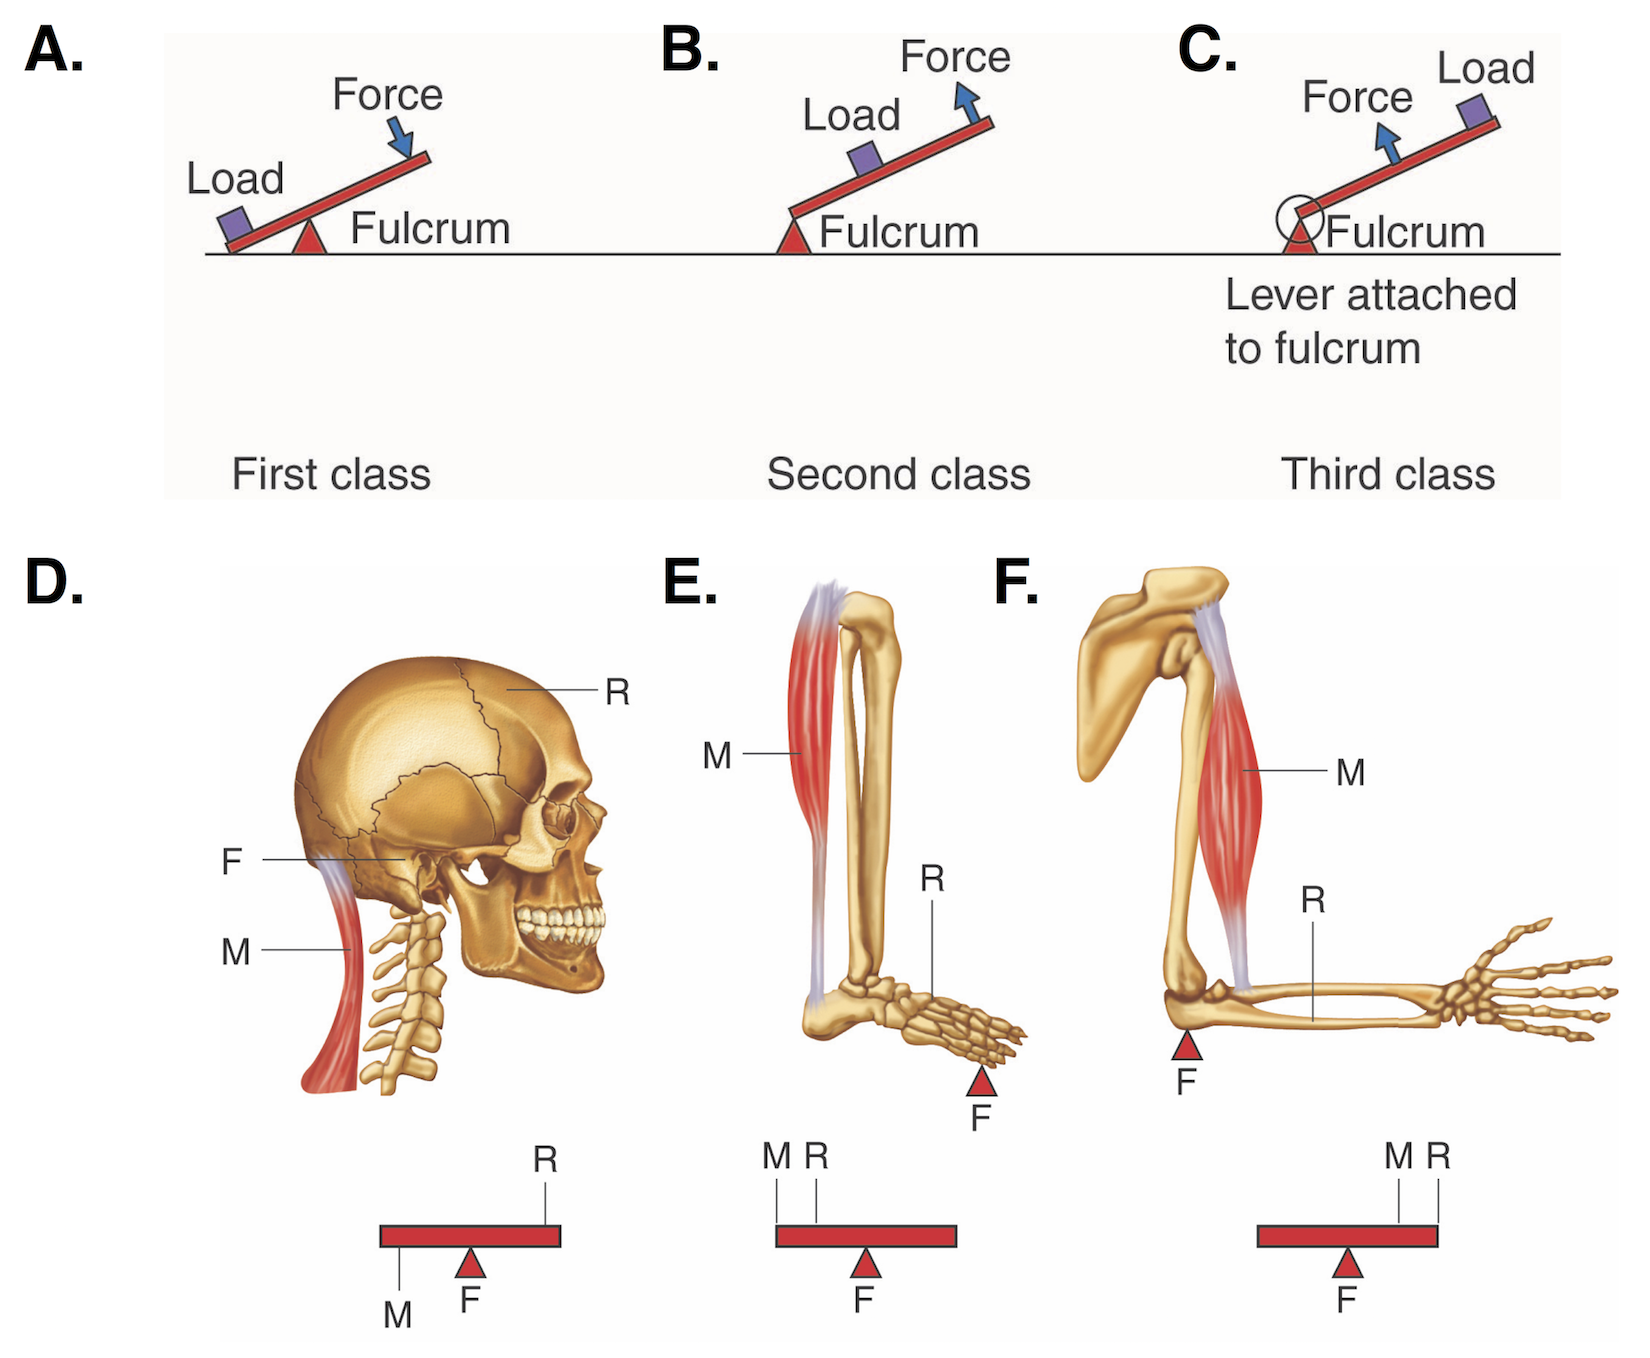
\includegraphics[width=0.95\textwidth]{figures/levers2.png}
\caption{Los tres clases de palancas (A-C.) y ejemplos de ellas en el
  cuerpo humano (D-F.). M - musculo, F - fulcro, and R -
  resistencia. Crédito del imagen: Open Learning Initiative
  \cite{leversOLI}, CC BY.}
\label{fig:levers}
\end{figure}

En el cuerpo humano, los huesos actúan como brazos de palanca y las
articulaciones como fulcros. La fuerza para superar una resistencia o
levantar una carga es proporcionada por la contracción de los músculos
esqueléticos, que están unidos a los huesos por tendones
\cite{leversOLI,openStax2016lever}. Las tres clases de palancas se
encuentran en el cuerpo humano, aunque algunas son más comunes que
otras \cite{leversOLI}. Las palancas de clase 1 son raras, pero
algunos ejemplos sí existen, incluyendo el sistema de
\emck{bone-joint} articulación ósea responsable de la flexión y
extensión de la cabeza (bajando o levantando la cabeza,
respectivamente; Fig. \ref{fig:levers}D).  En este caso, el fulcro es
la articulación entre el cráneo y el primer vertebra cervical. La
carga, o resistencia, es el peso de la cabeza sí mismo. La fuerza para
levantar la cabeza se aplica mediante la contracción de músculos
esqueléticos en el cuello y la parte superior de la espalda, incluido
el esplenio capitis y semispinalis capiti \cite{openStax2016axial}.
El brazo de palanca en este caso no es tan obvio como en los sistemas
de huesos largos \emck{long-bone systems}, pero es el cráneo en sí. Se
puede imaginar una línea corriendo diagonalmente desde los músculos
del cuello en el lado izquierdo, hacia arriba a través de la articulación
cervical, y terminando en un punto en el cráneo sobre la cuenca del
ojo.

Cuando una persona se pone de puntillas, podemos ver un ejemplo de una
palance de clase 2 en el cuerpo humano (Fig. \ref{fig:levers}E)
\cite{leversOLI}. El pie es el brazo de la palanca, las articulaciones
entre los huesos del pie y los de los dedos (las articulaciones
metatarsofalángicas) actúan como el fulcro, y la carga es el peso del
cuerpo de la persona. La fuerza requerida para levantar el cuerpo es
proporcionada por la contracción de los músculos gastrocnemio y sóleo
en la parte posterior de la pierna.

Las palancas de clase 3 son el tipo más común que se encuentra en el
cuerpo humano \cite{leversOLI}. El ejemplo clásico es el complejo
formado por el bíceps braquial, el codo y el antebrazo. En este
ejemplo, el antebrazo es el brazo de palanca, la articulación del codo
es el fulcro, y la fuerza requerida para mover el brazo hacia arriba
(flexión) o levantar una carga es proporcionado por el bícep.


\subsection*{Estructura de los músculos esqueléticos}

Para entender cómo se contraen los músculos, primero debemos conocer
su estructura. Los músculos esqueléticos se componen de múltiples
fascículos, que son paquetes \emck{bundles?} de muchas fibras
musculares más pequeñas rodeadas por una capa de tejido conectivo (el
perimisio) \cite{openStax2016muscle}. En muchos músculos esqueléticos,
los fascículos están alineados paralelos entre sí, corriendo a lo
largo del longitud del músculo \emck{running the length of?}
\cite{openStax2016lever}. \emck{Other muscles show a circular fascicle
  arrangement. Some muscles have fascicles which meet at one
  attachment point (convergent), while others feather out from a
  central tendon (pennate). The arrangement of the fascicles affects
  the direction and angle at which the fibers can pull, and also
  affects force generation in the muscle} Otros músculos muestran un
arreglo circular de fascículos. Algunos músculos tienen fascículos que
se encuentran en un accesorio punto (convergente), mientras que otros
se pliegan desde un tendón central (pennate). La disposición de los
fascículos afecta la dirección y ángulo al que las fibras pueden
tirar, y también afecta la generación de fuerza en el músculo
\cite{openStax2016lever}.

Cada fibra muscular está compuesta de muchas miofibrillas más
pequeñas, que contienen la maquinaria molecular para la contracción
\cite{openStax2016muscle}. Alrededor de la fibra muscular es la
membrana plasmática o sarcolema. En el sarcolema se encuentran
proteínas transmembranas integradas, como los canales iónicos que
median las corrientes y permiten la generación de los potenciales de
acción (APs) en músculo \cite{openStax2016muscle}. Estos APs se
propagan a través de invaginaciones en la sarcolema, conocidos como
túbulos transversales (T-túbulos;
Fig. \ref{fig:ttubules}). Posicionado justo al lado de los T-túbulos
es el retículo sarcoplásmico, el equivalente del retículo endoplásmico
en músculo. Aquí, canales selectos responden a los cambios en el
voltaje generados por la propagación de los APs para iniciar eventos
intracelulares que activan la maquinaria contráctil
\cite{openStax2016muscle}.


\vspace{0.2cm}

\begin{figure}[h!]
\centering
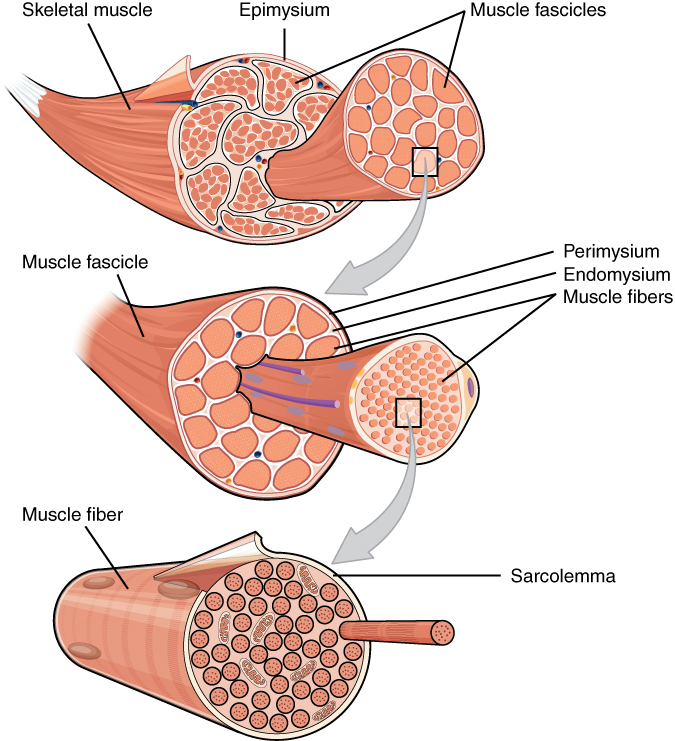
\includegraphics[width=0.7\textwidth]{figures/muscleStructure.jpg}
\caption{Estructura de músculo y niveles de organización. The top
  image shows the muscle fascicles. La imagen superior muestra los
  fascículos musculares. La siguiente imagen hacia abajo se acerca
  \emck{zooms in on?} un fascículo para mostrar las fibras
  musculares. La imagen inferior se acerca a una fibra muscular
  para mostrar las miofibrillas. Crédito de la imagen: OpenStax
  \cite{openStax2016muscle}, CC BY.}
\label{fig:fibers}
\end{figure}

\vspace{0.2cm}

\begin{figure}[h!]
\begin{minipage}{.45\textwidth}
\centering
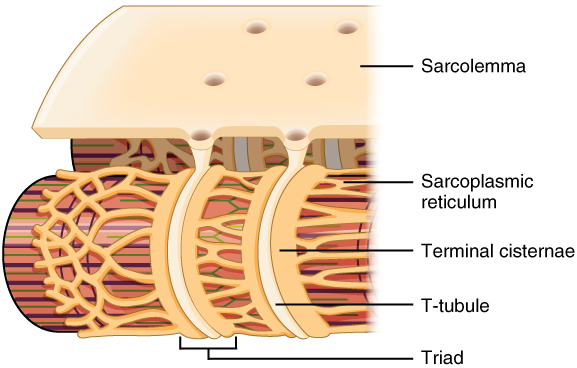
\includegraphics[width=0.95\textwidth]{figures/T-tubule.jpg}
\end{minipage}%
\begin{minipage}{.52\textwidth}
\centering
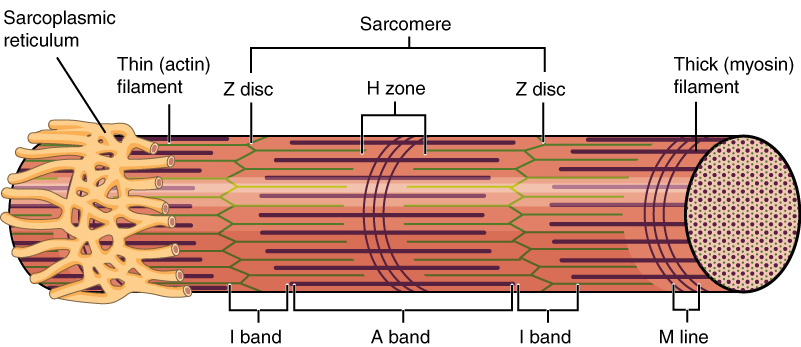
\includegraphics[width=0.95\textwidth]{figures/SRsarcomere.png}
\end{minipage}
\caption{\textit{Izquierdo}: Las invaginaciones en el sarcolema forman
  los T-túbulos, que descienden por las miofibrillas y están
  flanqueados por el retículo sarcoplásmico (SR) en ambos lados.
  \textit{Derecho}: Cerca del SR, las proteínas están organizadas en
  sarcómeros, la unidad contráctil del músculo. Diferentes zonas
  están delineadas dentro del sarcómero por la presencia y
  superposición de proteínas y filamentos selectos. Crédito de
  la imagen: OpenStax \cite{openStax2016muscle}, CC BY.}
\label{fig:ttubules}
\end{figure}

La unidad contráctil funcional del músculo esquelético se conoce como
el sarcómero \cite{openStax2016muscle}. En los músculos esqueléticos,
sarcómeros están organizados en serie a lo largo de las
miofibrillas. Cambios regulares y repetidos en la densidad de proteínas
particulares en los sarcómeros es lo que le da a los músculos
esqueléticos su apariencia rayado, o estriado, bajo un microscopio.

\subsection*{Modelo de los filamentos deslizantes y relación longitud-tensión}
Los sarcómeros contienen varias proteínas, como la titina, que actúan
como un ``resorte molecular'' y es importante para establecer la
elasticidad y tensión pasiva en los músculos \cite{granzier2006giant}.
Sin embargo, la base de la contracción radica \emck{lies in?} en la
interacción entre los filamentos de actina (delgados) y filamentos de
miosina (gruesos) \cite{openStax2016contraction}. Estos filamentos
están ordenados \emck{organizados?} en paralelo, con áreas de
superposición \emck{translape?}. La miosina puede unirse a la actina a
través de sitios de unión en la región de la cabeza de miosina,
formando lo que se llaman puentes cruzados. Cuando la cabeza se mueve,
esto hace que los filamentos se deslizan uno tras otro, aumentando el
área de superposición y acortando el sarcómero. Cuando esto sucede en
múltiples sarcómeros a lo largo de la longitud de la miofibrilla, la
miofibrila se acortan. Si el mismo efecto ocurre en muchas
miofibrillas en muchos fascículos, todo el músculo se acorta y produce
una contracción. Esta descripción de la interacción del filamentos de
miosina y actina se llama el modelo de filamentos deslizantes de
contracción. Los pasos por los cuales los filamentos de miosina y
actina se enganchan, deslizan, desengranar, y luego reinician
\emck{reset?} se llaman colectivamente el ciclo de puentes cruzados
\cite{openStax2016contraction} (discutido en más detalle abajo).
  
\vspace{0.2cm}

\begin{figure}[h!]
\centering
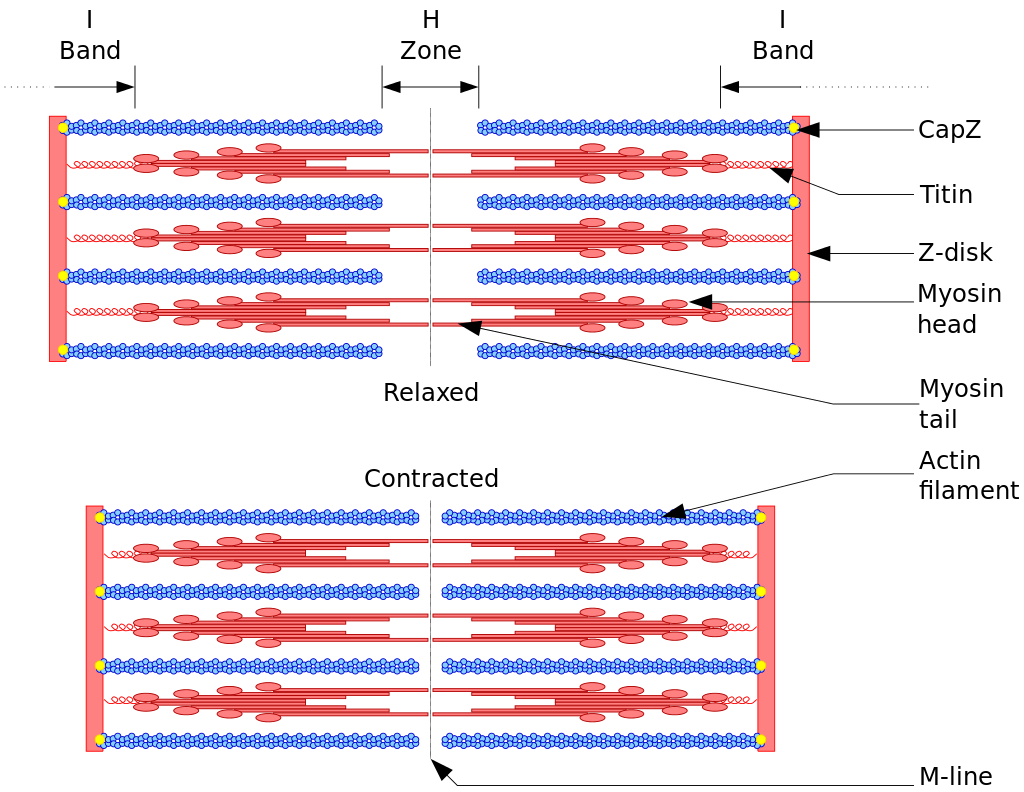
\includegraphics[width=0.8\textwidth]{figures/sarcomere.png}
\caption{Modelo de filamentos deslizantes de la contracción
  muscular. La imagen superior muestra un sarcómero en un músculo
  relajado. Los filamentos tienen áreas de superposición, pero no
  están activamente involucrados \emck{engaged?}. La imagen inferior
  muestra un sarcómero en un músculo contraído. Las cabezas de miosina
  se unen a los filamentos de actina, se mueven hacia el interior
  hacia la línea M, y deslizen para acortar el sarcómero. Credito de
  imagen: David Richfield \cite{richfieldSarcomere}, CC-BY-SA-3.0.}
\label{fig:sarcomere}
\end{figure}

\vspace{0.2cm}

Existe un nivel intermedio óptimo de superposición de filamentos que
produce la tensión máxima en el músculo \cite{openStax2016nervous}.
Tan poca superposición y los filamentos no se pueden unir e
interactuar; demasiado superposición y no hay capacidad para
deslizamiento adicional de los filamentos. La relación entre la
superposición de los filamentos (es decir, la longitud del sarcómero)
y la tensión muscular se llama la relación de longitud-tensión, y se
muestra en Fig.\ref{fig:tension}.

\vspace{0.2cm}

\begin{figure}[h!]
\centering
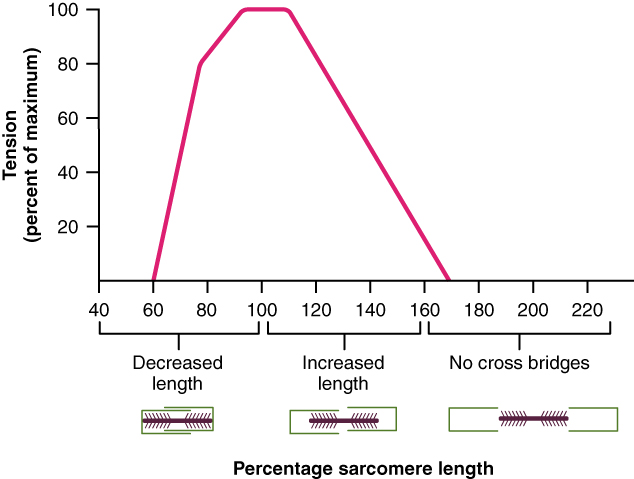
\includegraphics[width=0.75\textwidth]{figures/lengthTension.jpg}
\caption{Relación longitud-tensión en el músculo. La tensión máxima se
  produce cuando los filamentos de actina y miosina tienen una
  superposición óptima para deslizamiento, es decir, alrededor del
  80-120\% de la longitud del sarcómero en reposo. Crédito de la
  imagen: OpenStax \cite{openStax2016nervous}, CC BY 4.0}
\label{fig:tension}
\end{figure}

\subsection*{Acoplamiento de excitación-contracción y el ciclo de puentes cruzados}
Entonces, ¿cómo es que un potencial de acción (AP) generado en la
unión neuromuscular (NMJ) \footnote {La generación de potenciales de
  acción en el NMJ no es discutido aquí, pero puede ser revisado en
  Cap. 7 de \cite{guyton20006textbook}.} conduce a \emck{cross-bridge
  cycling} dentro del sarcómero. En otras palabras, ¿cómo se acopla la
excitación con contracción? El AP se propaga desde el NMJ hacia abajo
a través de los T-túbulos para llegar al interior de las miofibrillas
\cite{openStax2016contraction}. Dentro del túbulo T, el cambio en
voltaje activa un canal de calcio dependiente de voltaje conocido como
Ca$_{v}$1.1, o el receptor de dihidropiridina (DHPR)
\cite{schneider2012skeletal}.  El DHPR es mecánicamente vinculado al
receptor de rianodina (RyR) insertado en la membrana del retículo
sarcoplásmico (SR). La activación del DHPR causa un cambio
conformacional que, a su vez, activa RyR, abriendo el canal y
permitiendo que el calcio salga de la SR por su gradiente
electroquímico \cite{schneider2012skeletal}. Este aumento en el calcio
libre intracelular, a su vez, permite la formación de puentes
cruzados. Si el calcio no está presente, los puentes cruzados no
pueden formarse porque un complejo de proteinas tropomiosina y
troponina bloquea el sitio de unión de la miosina en los filamentos de
actina. Cuando el calcio se une a la troponina, da como resultado un
cambio conformacional que mueve la tropomiosina fuera del camino y
permite unir miosina y actina \cite{openStax2016contraction}. Una vez
que están unidos, los filamentos pueden deslizarse.

Para continuar con el ciclo, los filamentos de miosina y actina
también deben poder desvincular y restablecer su posición. Este
proceso requiere el aporte de energía en forma de ATP
\cite{openStax2016contraction}.

Cuando la miosina se une con ATP, se separa de la
actina. Posteriormente, el ATP está hidrolizado y la energía liberada
se utiliza para mover la cabeza de miosina de vuelta a la posición de
\emck{``cocked''}, listo para unirse con actina. ADP y un fosfato
inorgánico permanecen unidos a la cabeza de miosina. Entonces, la
miosina se une a la actina y libera el fosfato inorgánico. Luego, la
cabeza de miosina libera el ADP y se mueve hacia adentro en lo que se
llama el golpe de poder \emck{power stroke}, que hace que los
filamentos de actina se deslizen hacia la línea media y acortan el
sarcómero. El ciclo de puentes cruzados continúa siempre cuando haya
suficiente ATP y calcio. El músculo se relaja cuando el calcio se
bombea nuevamente al SR y ya no está disponible, permitiendo que la
tropomiosina bloquea el sitio de unión de actina-miosina una vez más
\cite{openStax2016contraction}.

\textbf{Pregunta de estudio:} ¿Cómo es que las detalles moleculares
del acoplamiento excitación-contracción difieren en músculo
cardíaco y liso, en comparación con músculo esquelético?

\subsection*{Respuestas de la fibra muscular, suma y reclutamiento}

La respuesta de un músculo a la estimulación (ya sea externa o interna
a través de la entrada sináptica) depende del tiempo y la fuerza del
estímulo \cite{openStax2016nervous}. Si solo ocurre un breve estímulo,
entonces una fibra muscular responderá con un solo AP y solo se
producirá una contracción corta (de decenas a cientos de
milisegundos). Porque los eventos intracelulares necesarios para
producir una contracción toman más tiempo que aquellos que generan un
AP, otro AP puede llegar antes que la fibra muscular se ha relajado
por completo. Si esto ocurre, la segunda respuesta se agregará a la
tensión ya presente en el músculo en un proceso llamado suma
\emck{summation?}. Alcanzar la contracción sostenida de la fibra
muscular y generar la tensión lo suficientemente grande como para
hacer trabajo requiere la suma de múltiples eventos estimuladores.

Además de la suma dentro de las fibras músculares individuales,
múltiples fibras se activan para lograr la contracción al nivel del
músculo completo. Una neurona motora y todas las fibras musculares a
las que envía señales (inerva) dentro de un músculo se llama una
unidad motora. Las unidades motoras pueden variar en tamaño, con
algunas neuronas motoras inervando pocas fibras (unidad pequeña) y
otras inervando muchas (unidad grande). Los músculos pueden variar
la fuerza que generan dependiendo del número y tipo de unidades
motoras que están activadas (reclutadas).

\vspace{0.2cm}

\begin{figure}[h!]
\begin{minipage}{0.45\textwidth}
\centering
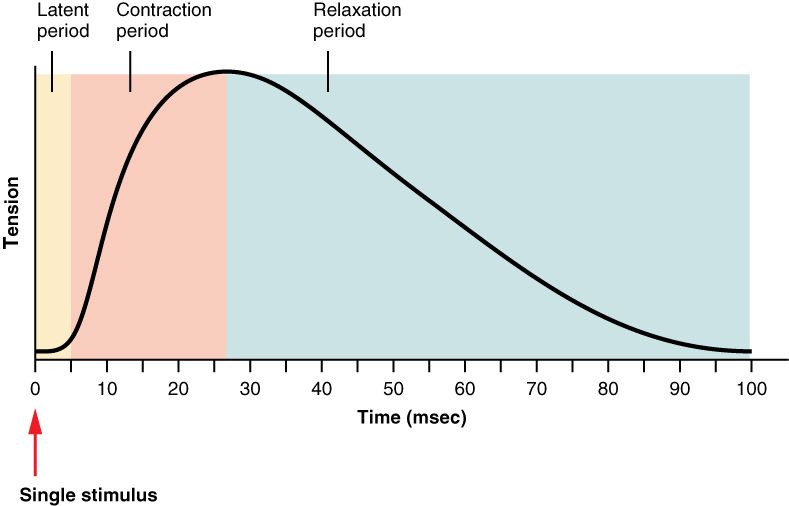
\includegraphics[width=0.95\textwidth]{figures/myogram.jpg}
\end{minipage}%
\begin{minipage}{0.55\textwidth}
\centering
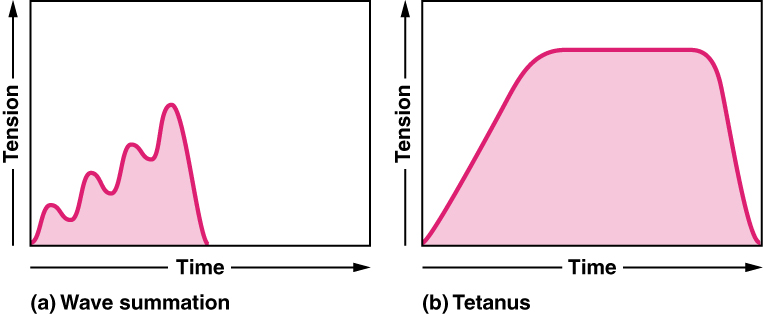
\includegraphics[width=0.95\textwidth]{figures/summation.jpg}
\end{minipage}
\caption{Respuestas musculares \textit {Izquierda:} Miograma que
  muestra la tensión desarrollada durante una contracción corta de una
  fibra muscular resultando de una sola, breve
  estímulo. \textit{Derecha:} Múltiples estímulos entregados en
  sucesión rápida produce suma y aumenta la tensión. Si la frecuencia
  de la estimulación es lo suficientemente alta, las respuestas se
  fusionan en el tétano. Tensión máxima y una contracción suave se
  logra. Credito de imagen: OpenStax \cite{openStax2016nervous}, CC
  BY.}
\label{fig:twitch}
\end{figure}

\subsection*{Medición de la actividad eléctrica de los músculos esqueléticos - electromiograma}

Para registrar la actividad eléctrica de los músculos usamos una
técnica llamada electromiografía, y los registros que obtenemos se
llaman electromiogramas (EMGs) \cite{garcia2011surface}.

Grabación EMG puede ser hecho de forma invasiva mediante la inserción
de electrodos en el músculo de interés, o de forma no invasiva
mediante el uso de electrodos de superficie colocados en la piel
arriba del músculo (Fig. \ref{fig:emg}). La inserción de electrodos
tiene la ventaja de dar registros EMG más ``limpios'' en los cuales la
actividad de unidades motoras separadas se puede distinguir. Sin
embargo, la inserción del electrodo puede ser doloroso y requiere
condiciones estériles para prevenir la infección, haciendo que este
tipo de registro no es ideal para el ambiente de aula. Electrodos de
superficie, por el contrario, pueden aplicarse y retirarse fácilmente
de la piel sin lesiones. Las limitaciones de este tipo de registro
extracelular incluye solo poder registrar de músculos superficiales, y
registros que muchas veces no permiten la separación de unidades
motoras individuales \cite{garcia2011surface}.

Estas limitaciones no son prohibitivas y son típicamente
\emck{outweighed} por los beneficios de lo no invasivo
(\emck{non-invasiveness}), pero deben de tomar en cuenta cuando
pensamos de la ubicación de electrodos y análisis de datos.

Una de las configuraciones de registro más comunes se conoce como EMG
bipolar, o EMG sensillo diferencial \cite{garcia2011surface}. Dos
electrodos de superficie están colocados en la piel sobre el músculo
separados por pocos centimetros (Fig. \ref{fig:emg}). Restando las dos
señales registrados en los dos puntos y después amplificando la
diferencia, señales comunes que pueden resultar de músculos fuera del
sitio de registro están \emck{largely?} excluidas, and principalmente
cambios locales en actividad están registrados. POr lo tanto, este
configuración disminuye \emck{cross-talk?} muscular
\cite{garcia2011surface}.

\begin{figure}[h!]
\centering
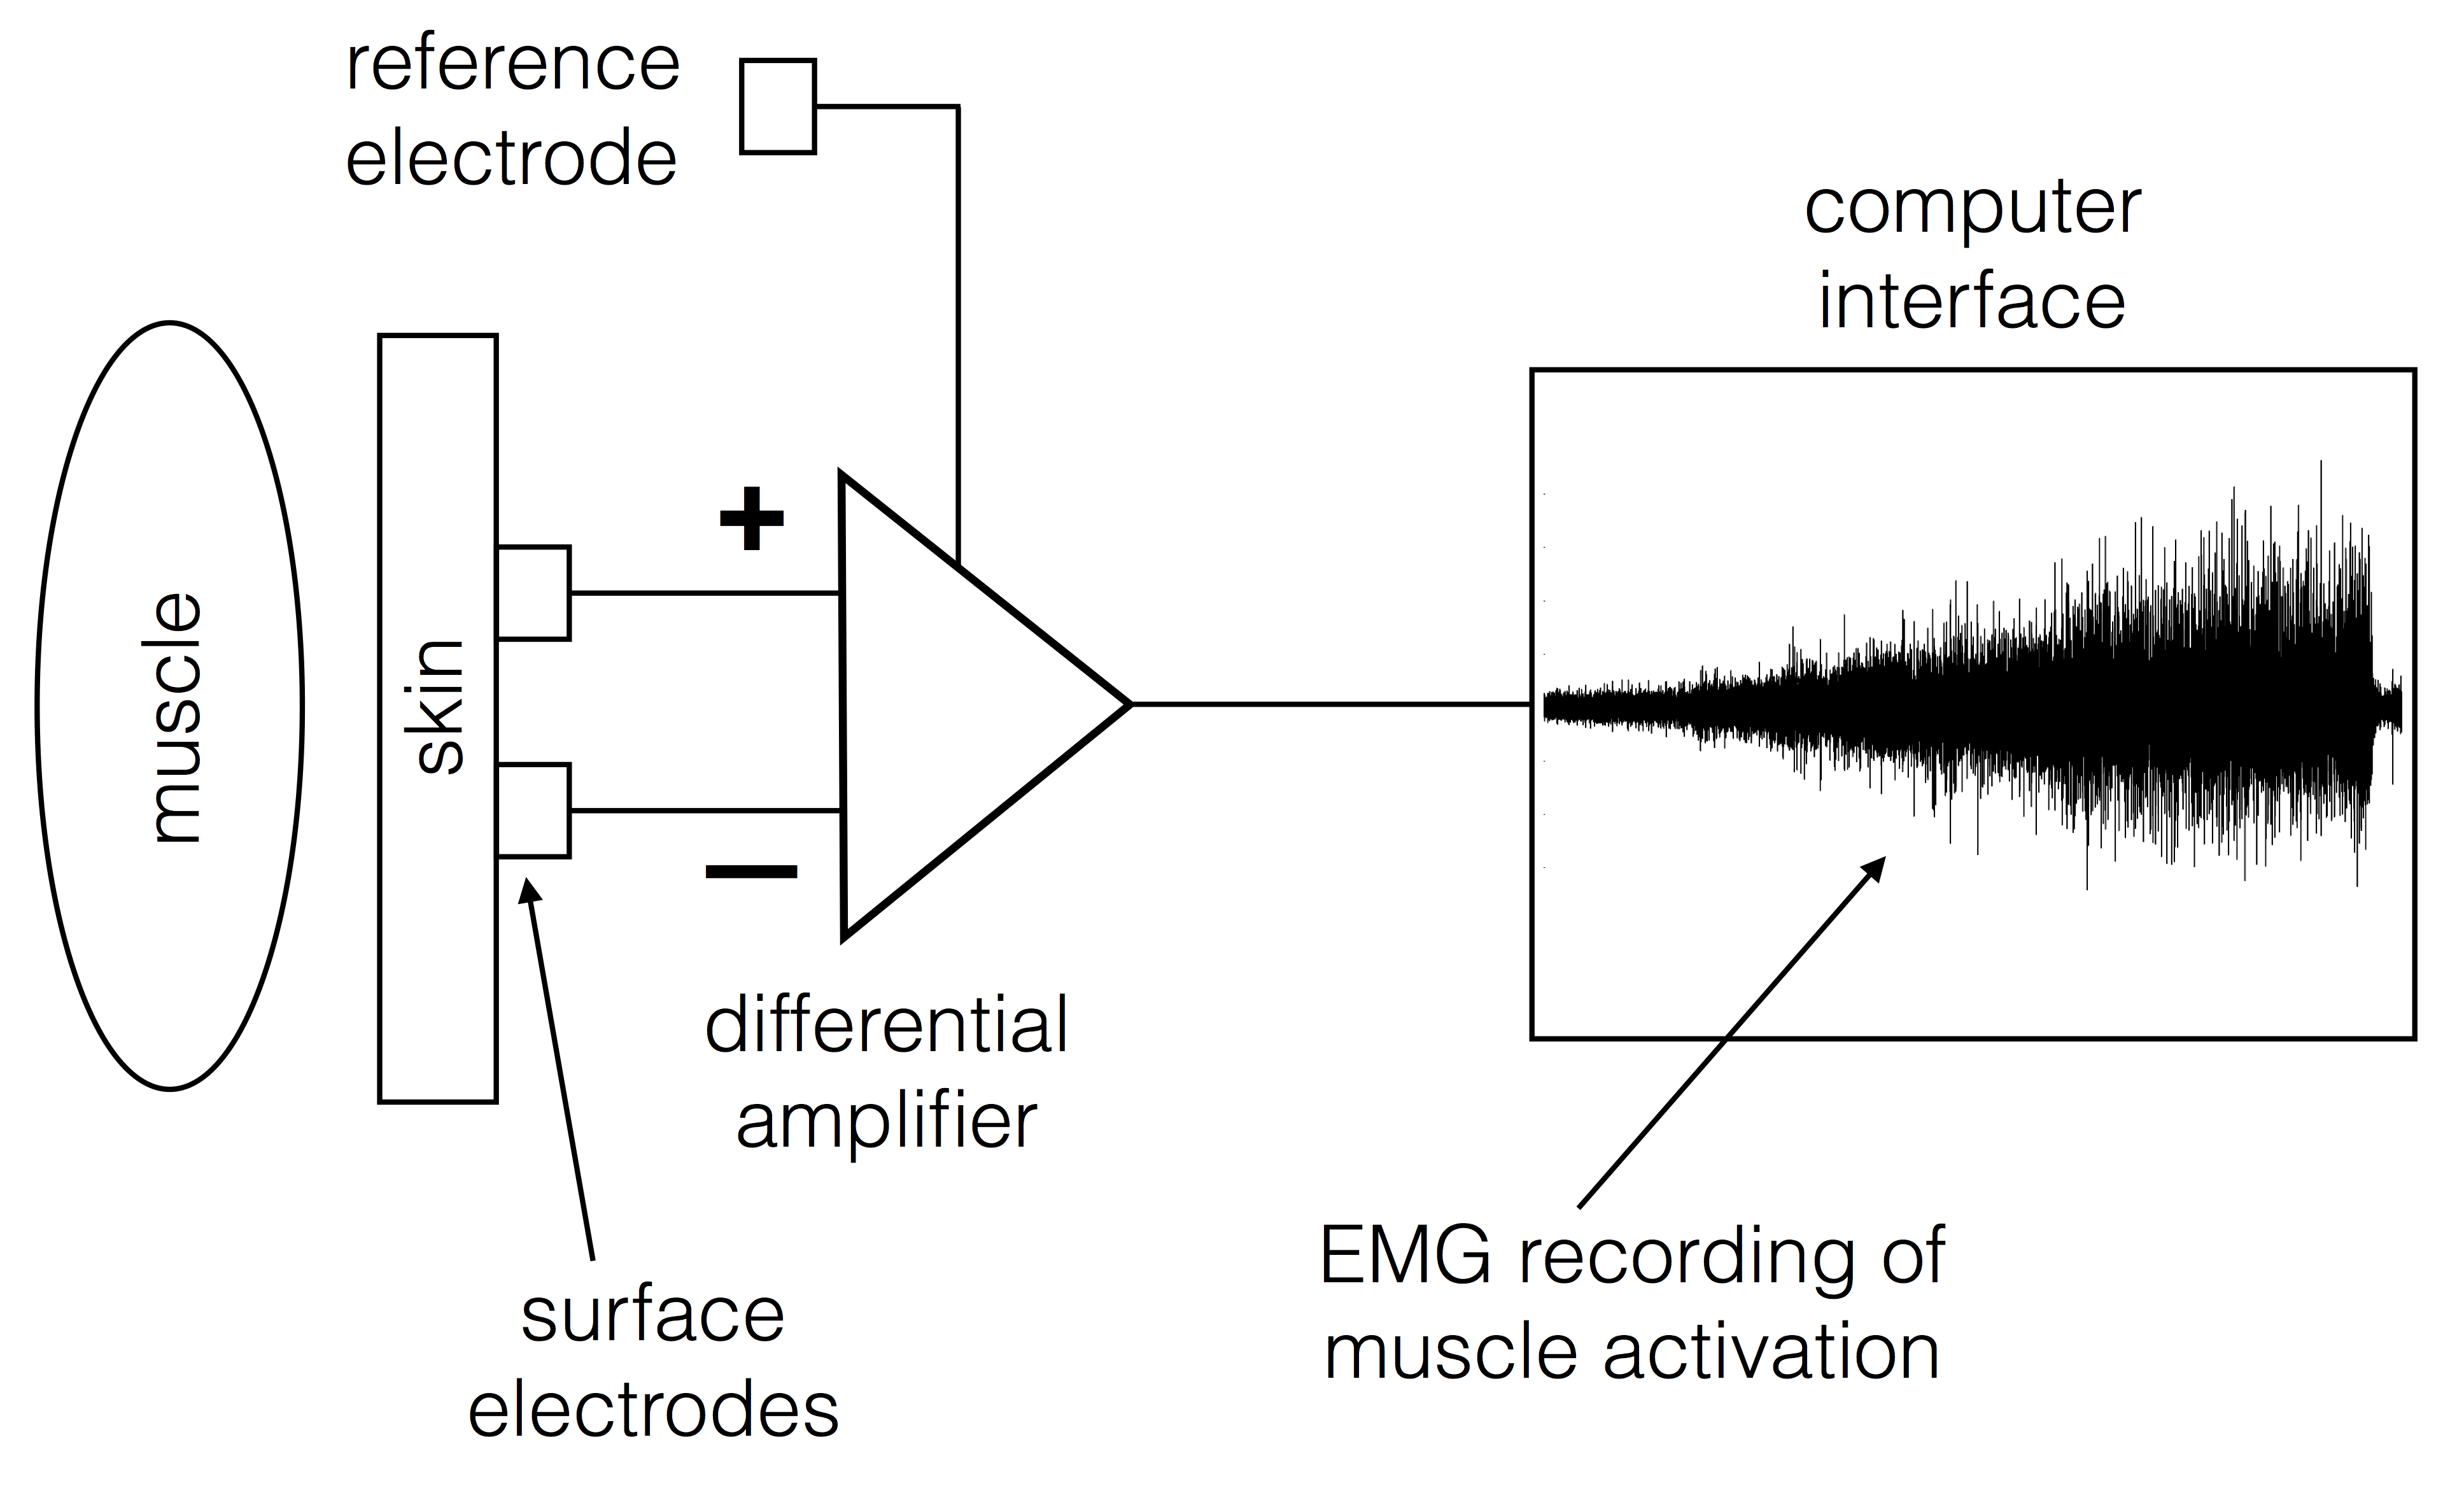
\includegraphics[width=0.7\textwidth]{figures/emgAmp.png}
\caption{Configuración EMG bipolar. Por simplicidad, no todos los
  componentes del cuerpo o registro se muestran. Crédito: Erin
  C. McKiernan, CC BY.}
\label{fig:emg}
\end{figure}

EMGs bipolares de superficie nos pueden decir varias cosas sobre
actividad muscular \cite{garcia2011surface}. Uno es el curso temporal
de la activación y relajación de los músculos. La mayoría de los
músculos muestran muy poca actividad cuando están en reposo. Cuando se
activan, vemos un incremento notable en la ocurencia \emck{?} de kis
impulsos eléctricos, como muestra en la Fig. \ref{fig:emg} (lado
derecho). Cuando el músculo se relaja, estos impulsos desaparecen y
registramos solo el ruido de base. El curso temporal de la actividad
muscular se puede despuñes correlacionar con otras medidas. También
podemos, hasta cierto punto, estimar la fuerz o esfuerzo exergido
durante una contracción. Mientras que el sujeto aumenta la fuerza de
contracción, vemos un aumento en la frecuencia de los impulsos
eléctricos y también la amplitud de la señal. Estos cambios resultan
de dos factores: (1) una frecuencia de disparo más alta en unidades
motoras ya activas, y (2) el reclutamiento de unidades motoras
adicionales. Acuerdanse, estamos registrando la actividad de multiples
unidades motoras. Con aumento en la fuerza de contracción, más
unidades motoras estñan recultadas y empiezan a disparar, su actividad
se suma, y contribuyen a los aumentos en la frecuencia y amplitud.

\subsection*{Preguntas de estudio} 
\begin{enumerate}
\item ¿Dónde se tendrán que colocar sus electrodos para registrar EMGs
  de sistemas de palanca clase 1, 2 y 3?
\item ¿Van a poder registrar de cualquier músculos que quieren en cada
  sistema de palance? ¿Por qué sí o no?
\item ¿Cómo van a saber si han colocado corectamente los electrodos?
\end{enumerate}

\section*{PROCEDIMIENTO}

Antes de comenzar, aseguranse de que tengan todo el equipo necesario y
han instalado el software de grabación de Backyard Brains en su
computador o teléfono inteligente. Los pasos siguientes \emck{will
  guide you} en configurar el equipo y hacer los registros.

\subsection*{1. Configurar los registros EMG}

La caja de Backyard Brains Muscle SpikerBox llega \emck{fully
  assembled} y listo para registrar ready. Solo tienen que conectar la
pila, los cables, y electrodos.

\vspace{0.2cm}

\begin{enumerate}
\item Conecta la pila de 9V a sus terminales en el Muscle SpikerBox
\item Conecta el cable azul/negro o verde a la entrada de computadora
  o teléfono inteligente correspondiente en el Muscle SpikerBox; nota
  que el cable para el teléfono inteligente es direcional, aseguranse
  que tengan el lado correcto insertado en el equipo
\item Conectar e otro lado del cable azul/negro o verde a su
  computador o teléfono inteligente
\item Conectar el cable naranja a su entrada correspondiente en el
  Muscle SpikerBox
\item Coloca los electrodos encima del músculo de interés, solo unos
  centimetros por separados y orientados en paralelo a las fibras
  musculares; acuerdanse, para registrar cada tipo de palance, tendrán
  que cambiar la colocación de los electrodos entre experimentos
\begin{itemize}
\item Palanca clase 1 - ejemplo de músculo de interés: splenius capitis
\item Palance clase 2 -  ejemplo de músculo de interés: gastrocnemius
\item Palanca clase 3 -  ejemplo de músculo de interés: biceps brachii
\end{itemize}
\item Conecta cada uno de los clips de caiman rojos en las terminales
  del cable naranja a uno de los electrodos de superficie; aseguranse
  de que los clips metálicos no tocan entre ellos y tratan de evitar
  \emck{entangling} los cables
\item Agarra el clip de caiman negro (referencia) en su mano, o
  conectalo a otro electrodo de superficie en la parte superior de su
  mano o otro area fuera del sitio de registro

\vspace{0.2cm}

\begin{figure}[h!]
\centering
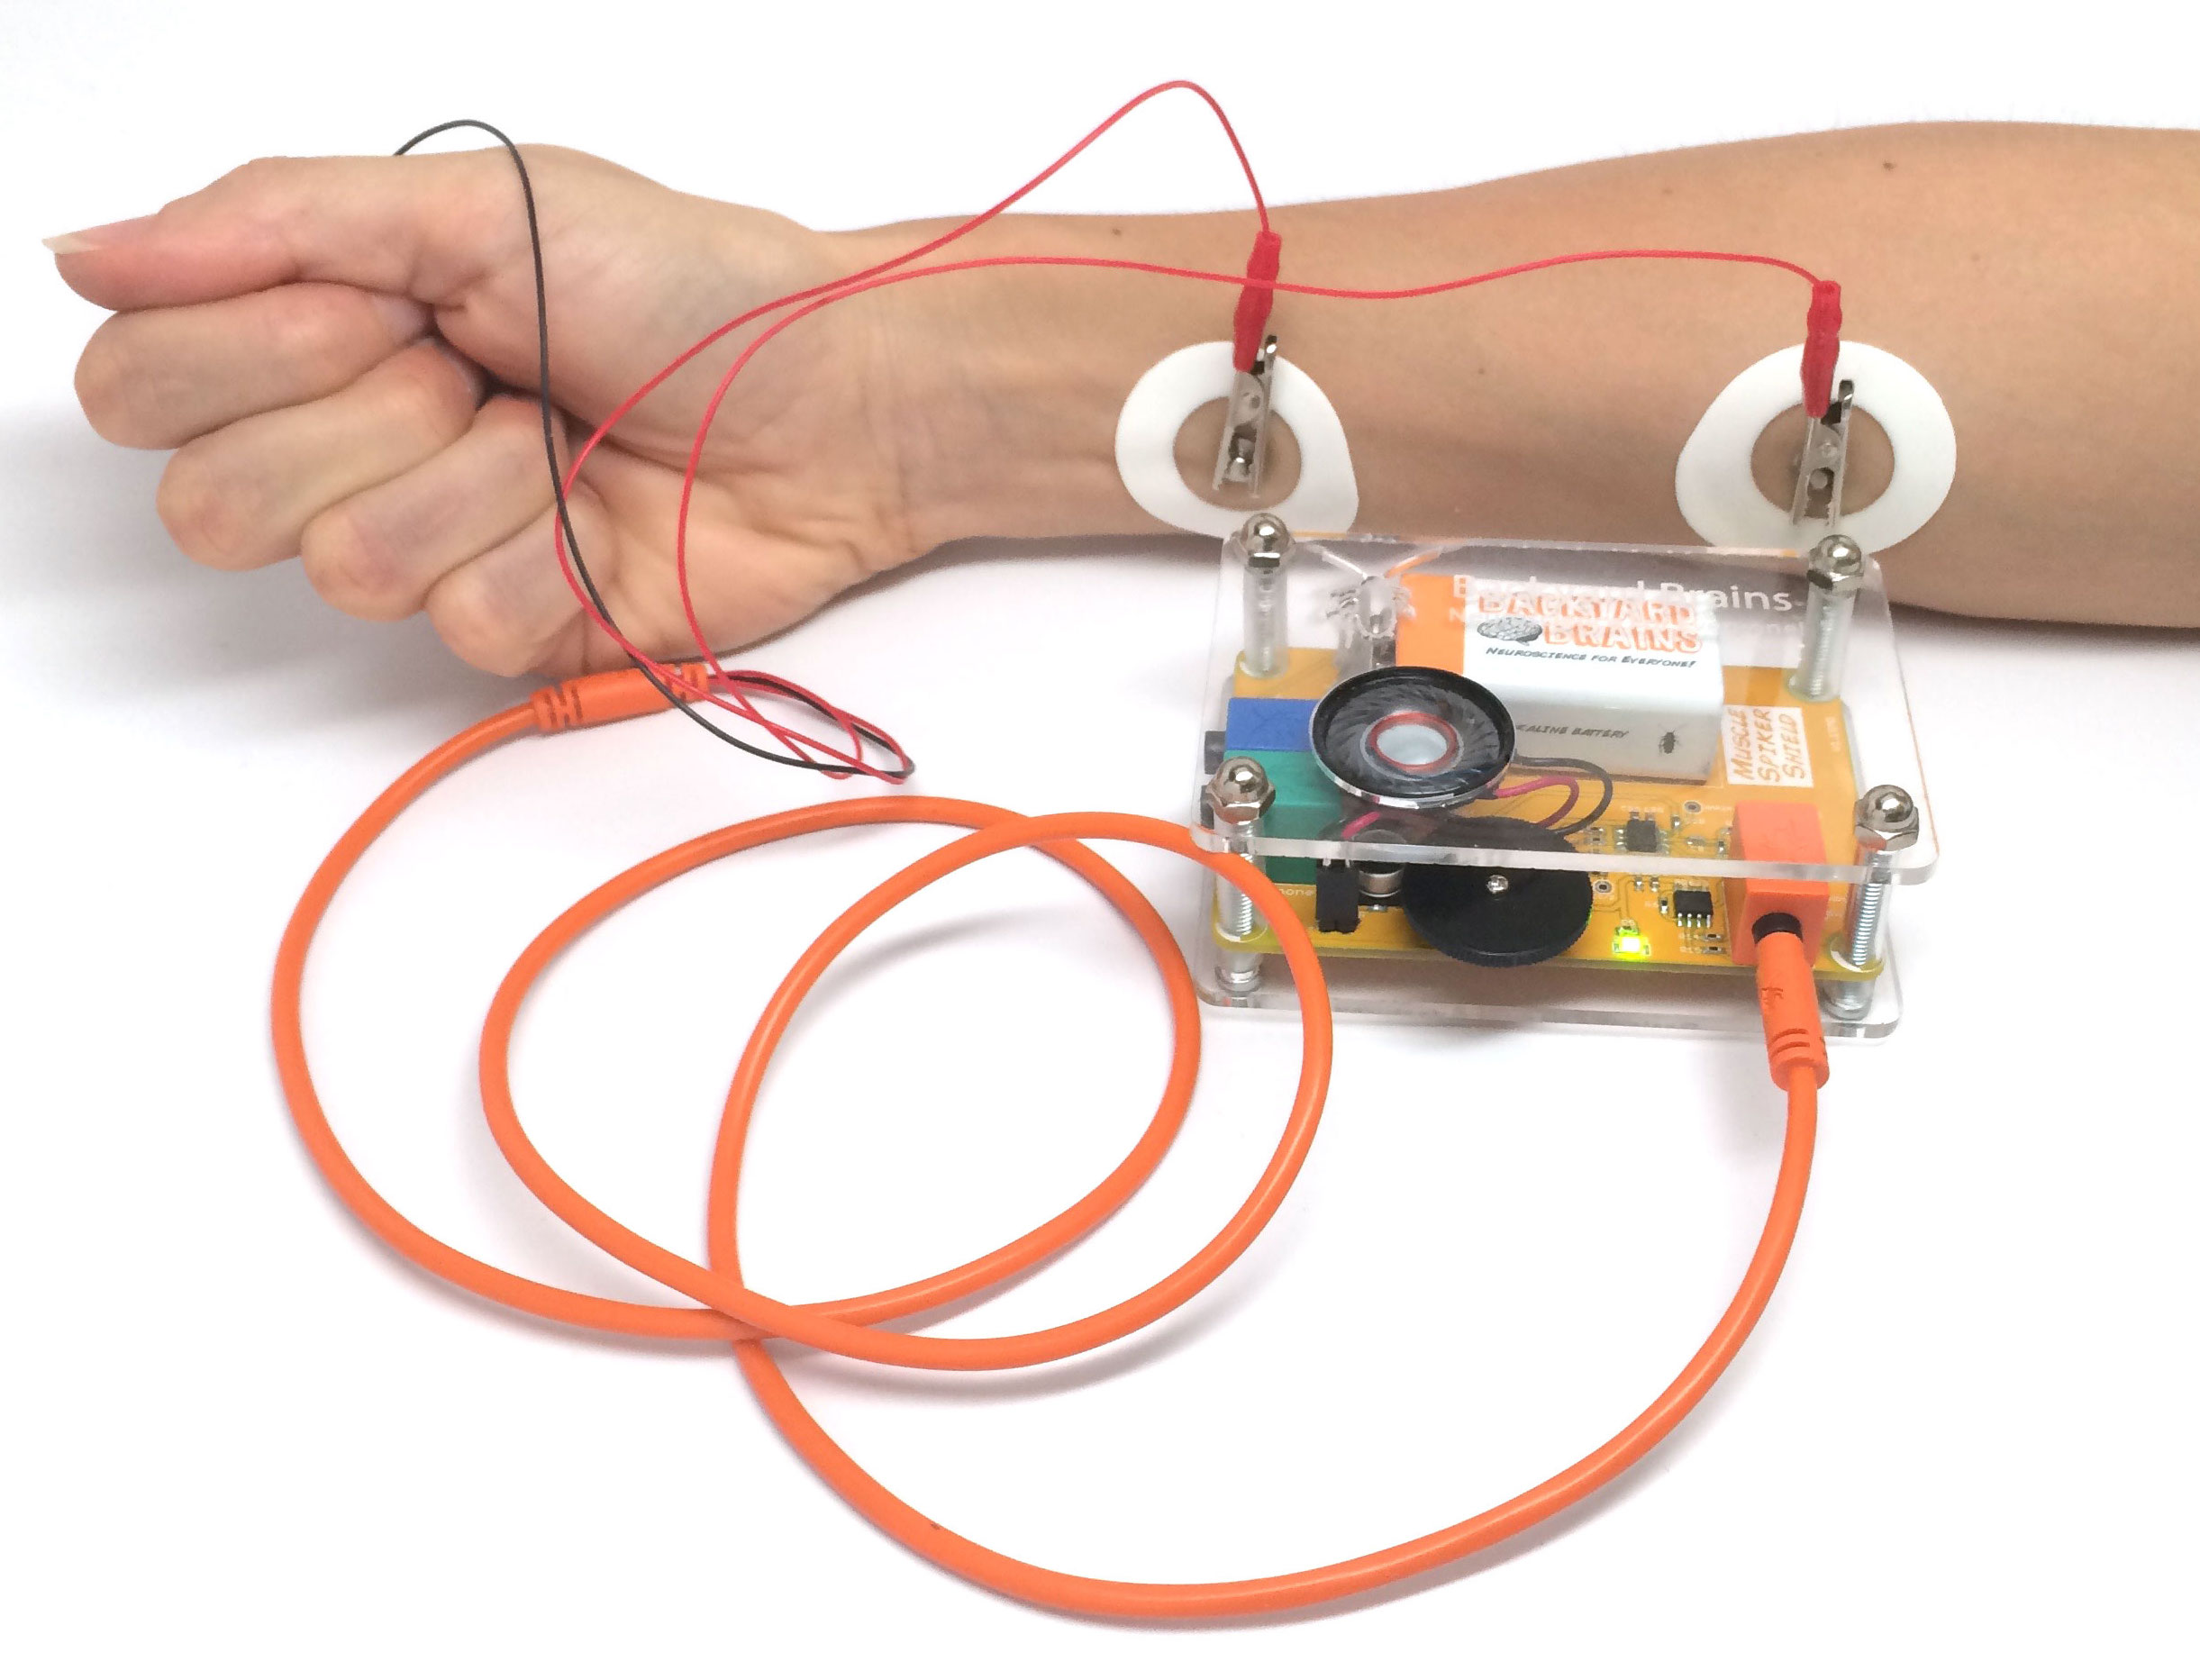
\includegraphics[width=0.8\textwidth]{figures/muscleSpikerBox.jpg}
\caption{\textit{Izquierdo}: Configuración de EMG con electrodos
  conectados al Muscle SpikerBox. (Connexión a computadora o
  teléfono inteligente no mostrado.) Crédito: Backyard Brains, CC BY SA.}
\label{fig:emgSetup}
\end{figure}

\item Para mejorar la señal de EMG, el área donde se colocarán los
  electrodos puede ser limpiado con alcohol antes de colocación;
  esperan hasta que el área se seca para poner los electrodos
\item Se puedes poner gel de electrodos puede para mejorar la
  conducción pero muchas veces no es necesario
\item Para evitar artifactos del ruido, aseguranse de que no hay ropa
  tocando los electrodos ni \emck{brushing} contra los cables durante
  el registro
\end{enumerate}
 
\subsection*{2. Poner a prueba los registros EMG}

\begin{enumerate}
\item Encienda el Muscle SpikerBox por rotar el \emck{wheel switch}
  negro ubicado en el lado de la caja, una luz verde debe de enceder;
  ¡tenga en cuenta que los electrodos deben estar conectados antes de
  encender el dispositivo y desconectados solo después de que el
  dispositivo esté apagado para evitar un ruido desagradable!
\item Abra el software de grabación Backyard Brains y explore los
  controles y configuraciones (para obtener más información sobre el
  uso del software, consulte \cite{spikeRecorder})

\begin{figure}[h!]
\centering
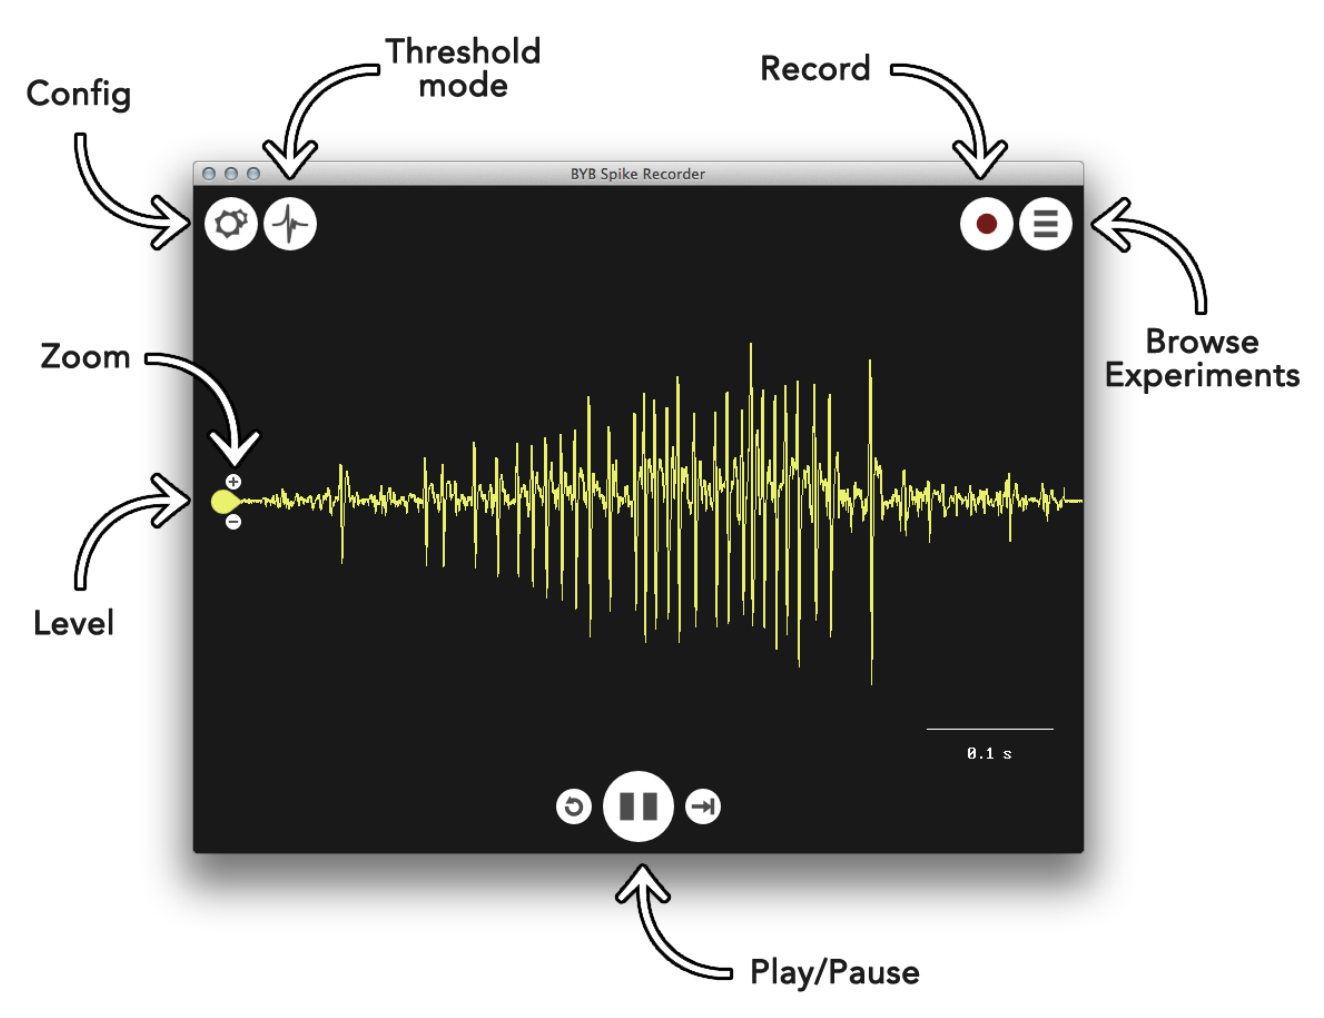
\includegraphics[width=0.8\textwidth]{figures/BBrecorder.png}
\caption{Interfaz de software de grabación. Crédito de imagen:
  Backyard Brains, CC BY SA.}
\label{fig:recorder}
\end{figure}

\item \emck{Snap?} sus dedos cerca del dispositivo de grabación; si
  ves un artefacto correspondiente en la pantalla, esto significa que
  estás registrando solo audio; para comenzar a registrar la actividad
  muscular, ajuste la configuración presionando el botón `Config '
  (Fig. \ref{fig:recorder}) (ve \cite{spikeRecorder} para más
  información)
\item Pídale al sujeto que brevemente contraiga y relaje el músculo de
  interés
\item Verifique que se observen potenciales eléctricos durante la
  contracción; checa tu relación señal / ruido; si la señal es
  demasiado pequeña, puede ajustar el \emck{gain?} girando el
  interruptor de la rueda (\emck{wheel switch?}) hacia la derecha
\item Intente guardar un registro en su computadora o teléfono
  inteligente (el formato será de .wav)
\end{enumerate}

\subsection*{3. Colectar sus datos}

\begin{enumerate}
\item Asegúrese de que la EMG esté listo para registrar y el sujeto
  está en posición de reposo
\item Antes de que comience el registro, haga que el sujeto piense en
  el tipo de movimiento que necesitan hacer para activar el músculo de
  interés, e.j., para el músculo gastrocnemio, esto involucrará
  poniéndose de puntillas, mientras que para el splenius capitis, esto
  implica levantar la cabeza
\item Cuando el sujeto esté listo, presione grabar en el interfaz de
  software de Backyard Brains
\item Indique al sujeto que permanezca relajado durante 3-5 segundos
  después de que comienza la grabación, luego contrae el músculo de
  interés para 3-5 segundos, y luego relajarse de nuevo por 3-5
  segundos
\item Haga que el sujeto repita la secuencia anterior al menos 3 veces
\item Termine los registros y guarde los datos en su computadora o
  teléfono inteligente
\item Los EMG deben guardarse y exportarse en formato .wav para su
  análisis
\item Comience un nuevo registro para examinar los efectos de la fuerza
  de contracción
\item Instruya al sujeto realizar la primera contracción con poca
  fuerza, luego hacer una pausa, luego realizar una segunda
  contracción con mayor fuerza, luego pausa, y finalmente realizar una
  tercera contracción con fuerza máxima
\item Termine los registros y guarde los datos en su computadora o
  teléfono inteligente
\item Comience un nuevo registrp para examinar la fatiga
\item Instruya al sujeto contraer el músculo de interés y
  mantener todo el tiempo que puedan; ¿Cuánto tiempo pueden
  sostenerlo? ¿Qué pasa cuando comienzan a cansarse? ¿Qué pasa si
  usan el mínimo versus la máxima fuerza?
\item Termine los registros y guarde los datos en su computadora o
  teléfono inteligente
\item Repita los pasos 1 a 13 para cada músculo que pertenece a los
  tres tipos de sistema de palanca; los sujetos deben descansar
  unos minutos entre sesiones de grabación
\item Recuerde etiquetar sus datos para que sepa a cual sujeto,
  músculo y tipo de experimento al que pertenece cada registro
\end{enumerate}

\section*{AGRADECIMIENTO}
Este trabajo fue apoyado por la Dirección General de Asuntos del
Personal Académico, Programa de Apoyo a Proyectos para la Innovación y
Mejoramiento de la Enseñanza en la Universidad Nacional Autónoma de
MéXico (UNAM-DGAPA-PAPIME clave PE213817).
 
% BIBLIOGRAPHY
\renewcommand\refname{REFERENCIAS}
\renewcommand{\markboth}[2]{}%
\begin{footnotesize}
\bibliography{EMG}
\end{footnotesize}

\end{document}
